\section{Introduction}

The statistician George Box famously said that 
``Essentially, all models are wrong, but some are useful.''
\citep{box1987empirical}.  
That is, by necessity, a statistical model is a simplification of the phenomenon
that it is modeling, and indeed, increasing fidelity is not always a
good thing.  For one, more complex models are more difficult to
understand, which can be important if the goal of modeling is to
achieve some insight about the law-like behavior governing a natural
phenomenon.  But even if the model is being applied strictly for the
purposes of making predictions, and being able to gain some verbal
understanding is not a priority, the more complex a model becomes, the
more sensitive it is to the idiosyncracies of the data that it is
informed by.

An important question in statistics is how to go about choosing a
model with enough complexity and flexibility to account for 
the interesting regularities in the process that produced the data, 
but not so much complexity that the model will not generalize; 
after all, the purpose of statistical
modeling is almost always to explain something and/or to make
predictions about the future, not simply to describe data already
collected.

A number of techniques have been developed in both frequentist and
Bayesian statistics to select from among a set
of model forms one that balances fit and generalizability, that is, to
do {\bf model selection}.  An alternative to model selection is to
employ a model form whose complexity is not fixed, but instead adapts
to become increasingly flexible as the data set grows larger: this is
the {\bf nonparametric} approach, which has a long history in
frequentist statistics (e.g., \cite{rosenblatt1956remarks,
  parzen1962estimation}), where the typical approach is to model the
data without any assumptions about the specific distributional family
that generated the observations.  

Distribution-free estimators have
been shown to have good asymptotic properties (see, e.g.,
\cite{wasserman2007nonparametric} for a review of the theory), but for finite
samples, usually require {\em ad hoc} ``smoothing'' parameters to be
specified by hand, or chosen using cross-validation.  In Bayesian
statistics, ``smoothing'' occurs naturally through the prior, but the
notion of a model with no distributional assumptions at all is not
particularly natural in a statistical approach that requires a well-defined
distribution to be specified over all possible data generating
processes.

In recent decades, however, and especially in the last decade, a field
of {\bf Bayesian nonparametrics} has grown up.  Bayesian nonparametric
models share with their non-Bayesian counterparts the property that
the flexibility of the model increases as the sample size increases,
but instead of being entirely distribution-free, Bayesian
nonparametric models employ countably infinite dimensional families of
distributions that can approximate large classes of distributions (e.g., all continuous
distributions) arbitrarily well
\citep{lindsay1995mixture,mclachlan2004finite}.  The result is to
combine the explicitness of assumptions in Bayesian models with the
flexibility of nonparametric models.

The central innovation in this dissertation is a new nonparametric
Bayesian model for sequence data, the Hierarchical Dirichlet
Process Hidden Markov Model with Local Transitions (HDP-HMM-LT, or
HaMMLeT, for short).  Hidden Markov Models (HMMs) are used to model
observed sequence data as ``noisy'' realizations of an underlying
sequence of discrete states.  The HaMMLeT model generalizes an existing model, the
Hierarchical Dirichlet Process Hidden Markov Model (HDP-HMM), by
allowing a metric structure to be specified on the state space of the
underlying Markov chain, providing a mechanism to build into the state
transition prior the notion that consecutive states are ``similar'' in
some way.

A challenge for most Bayesian modeling, not least inifinte-dimensional nonparametric
Bayesian modeling, is developing efficient algorithms to compute
(or approximate) desired functions of the posterior distribution,
since for all but the simplest models, explicit integration is
intractable.  For nonparametric models in particular, a key property of any
practical inference algorithm is that it must be able to represent
needed properties of the infinite-dimensional posterior using finite
storage and processing.  Thus, any time a new nonparametric model is
proposed, a central challenge is introducing a tractable and efficient
inference algorithm.  I present a simple Gibbs sampling algorithm
\cite{geman1984stochastic} to sample from the joint posterior of all
parameters and hyperparameters of HaMMLeT as well as the latent state
sequence, which is achieved by the introduction of a set of auxiliary
variables with a natural interpretation under an augmentation of the
stochastic process underlying HaMMLeT.

\subsection{An overview of the dissertation}
\label{sec:an-overv-diss}

In the remainder of this chapter, I begin by discussing the general
problem of model selection in the context of the bias variance
tradeoff, and how Bayesian models in particular provide a natural
Occam's Razor principle to balance fidelity to data on the one hand,
and simplicity on the other.  Then I introduce the finite dimensional
versions of the models on which HaMMLeT will build, namely mixture
models and their sequential counterparts, Hidden Markov Models.  In
Chapter \ref{chapter:HMM-NPBayes} I review the theory of Bayesian
nonparametrics, in particular Dirichlet Processes and Hierarchical
Dirichlet Processes, which underlie infinite mixture models and the
infinite-state Hidden Markov Model, respectively, and then define the
HDP-HMM of which HaMMLeT is a generalization.  In Chapter
\ref{chapter:HaMMLeT} I introduce the basic theory of HaMMLeT model
and an augmented stochastic process, the Markov Jump Process with
Failed Transitions, which provides an interpretable set of auxiliary
variables that greatly simplify posterior inference in HaMMLeT.  Then
in Chapters \ref{chapter:cocktail-party}-\ref{chapter:music} I define
some specific instantiations of HaMMLeT for a variety of kinds of
data, and give experimental results comparing HaMMLeT's inferential
performance to existing models.  Finally, in
\ref{chapter:discussion}, I give concluding thoughts and some
directions for future research.

\section{Model Selection}
\label{sec:model-selection}

\subsection{The Likelihood Function and the Conservation of
  Explanatory Power}
\label{sec:bayes-occams-razor}

In a parametric model family, $\mathcal{F} = \{f_{\theta}: \theta \in
\Theta\}$, the principle of maximum likelihood estimation can be seen
as choosing the parameter vector $\theta$ that makes the data as {\em unsurprising} 
as possible.  One consequence of this principle is that models that
are consistent with a broad range of possible data sets must spread
their predictive probability mass over a larger volume of possible
data, and thus assign a smaller probability (or probability density)
to any given data set.  When comparing the likelihood for a more
restrictive model to a more flexible model when both are consistent
with the data, then, the likelihood function will tend to prefer the
restrictive one.

To see a trivial example of this idea, consider the inference problem of
trying to decide what ``grammatical rule'' produced the following set of sequences:
\begin{align*}
  &{\sf lay\ lay\ dee} \\
  &{\sf way\ way\ dee} \\
  &{\sf fay\ fay\ dee}
\end{align*}
A few candidate rules are the following:
\begin{enumerate}
\item Any three syllables (call this the {\sf X Y Z} rule)
\item Any repeated syllable followed by another syllable (call this
  {\sf X X Y})
\item Any repeated syllable followed by the syllable {\sf dee} ({\sf X
    X dee})
\item Any repeated syllable rhyming with ``day'', followed by the
  syllable {\sf dee} ({\sf *ay *ay dee})
\item Three repetitions of the same syllable ({\sf XXX}).
\end{enumerate}

Which one seems to best describe the pattern?  All but the {\sf XXX}
rule are consistent with all three examples, but if we attribute a
probability model to each rule, by, for example, supposing that the
content of each ``free variable'' is chosen uniformly from the set of
viable candidates in the language, then we see that the {\sf *ay *ay
  dee} rule is the maximum likelihood choice, being the most
restrictive which is still consistent with the data.

In a sense, the likelihood principle exhibits the property of
{\em conservation of explanatory power}: a model has a total
probability mass that it can use to ``place bets'' on possible data
sets.  Models that allocate their probability mass over many data sets
are less likely to be categorically wrong, but do not get as big a
``reward'' as a model that distributes its bet over a smaller number
of possibilities.  Like betting on roulette, the ``vague'' bet on red
is reasonably likely to pay off, but results in a smaller profit than
the narrow bet on 34, which is much less likely to result in a payout,
but when it does, it is a large one.

This property of rewarding the most restrictive models acts as a form
of ``Occam's Razor'', which is the principle that states that all else
being equal we should prefer simpler explanations.  But although the
likelihood function rewards simpler (or at least more restrictive)
explanations in these toy examples of competing models with no free
parameters, it breaks down when competing models have differing
numbers of ``moving parts'', due to the problem of {\bf overfitting},
that is, of confusing the stochastic idiosyncracies 
in a particular data set (that is,
``noise'') for stable regularities in the data-generating process 
(that is, ``signal''). Since maximum
likelihood minimizes surprise, it will tend to give high scores to
models that are able to shift as much variability as possible away
from the stochastic noise component (which is surprising even after we
have settled on a model) and the deterministic signal component
(which, once we have a model, is not surprising).

\subsection{The Bias-Variance Tradeoff}
The notion of a tradeoff between model complexity and 
sensitivity to idiosyncracies in the data is formalized by the {\bf
  bias-variance tradeoff}.

Suppose that we have a model class, $\mathcal{F}$, and using
some data, $\{X,Y\}$, we will choose a specific model $\hat{f} \in \mathcal{F}$
that can be used to make a prediction about some future observation,
$y_{new}$ given some features, $x_{new}$.  That is, $\hat{f}(x_{new})$
yields some predicted value $\hat{y}_{new}$, which we want to be as
close as possible to the true but unknown value $y_{new}$.

Typically we cannot make perfect predictions, and there will be some
error, which we might quantify using squared distance:
\begin{equation*}
  \mathsf{Error}(x_{new}) = (\hat{f}(x_{new}) - y_{new})^2
\end{equation*}

Each dataset that we get yields a potentially different $\hat{f}$, and
thus a different error, and so we can consider the {\em expected}
error in prediction, or the {\bf mean squared error} (MSE)
\begin{equation*}
  MSE = \E{(\hat{f}(x_{new}) - y_{new})^2}
\end{equation*}
where the expectation is taken with respect to the true (but unknown) 
distribution of the data.

We can decompose the MSE as follows:
\begin{align*}
  MSE &= \E{(\hat{f}(x_{new}) - \E{\hat{f}(x_{new})} +
      \E{\hat{f}(x_{new})} - \E{y \given x_{new}} + \E{y \given
        x_{new}} - y_{new})^2}\\
    &= \V{\hat{f}(x_{new})} + (\E{\hat{f}(x_{new})} - \E{y \given
      x_{new}})^2 + \V{y_{new} \given x_{new}}\\
    &= \V{\hat{f}(x_{new})} + \mathsf{Bias}(\hat{f}(x_{new})) + \sigma^2_{\varepsilon}(x_{new})
\end{align*}
where the cross terms all cancel out.  The first term in the result
describes how much the prediction made by the fitted model varies
depending on the specific dataset used to choose $\hat{f}$.  The
second is the squared {\bf bias}, where the bias of a model is the
average discrepancy between its prediction and the truth.  Finally,
$\sigma^2_{\varepsilon}$ describes the unavoidable indeterminacy of
trying to make a prediction about $y_{new}$ using only $x_{new}$.
This last term does not depend on the choice of model class,
$\mathcal{F}$, but the bias and the variance do.

In general, the more complex the model class $\mathcal{F}$, the more
room it has to fit the true pattern of the data, and so the
greater its ability to be unbiased; however, this freedom often comes
at the expense of greater variance: even if on average the model class
yields a correct prediction, for a given dataset its prediction may be
farther away from that correct ``average behavior''.  This phenomenon,
of excessive sensitivity to idiosyncracies of the particular dataset,
is known as {\bf overfitting}.  On the other hand, we can trivially
produce a model with zero variance by using a constant prediction
regardless of the data; but this model is presumably going to have
greater bias, since unless $y_{new}$ is not related at all to the
input $x_{new}$, there will be values of the latter for which the
corresponding $y$ values are not centered around our constant
prediction (and even if the mean of $y$ is constant, we are unlikely
to be able to intuit this without using any data).

\subsection{Example: Polynomial Regression}
\label{sec:exampl-polyn-regr}

We can see the tradeoff between bias and variance (and the
consequences of overfitting) in the setting of
fitting a polynomial curve of order $d$ to a set of bivariate data.
In Fig. \ref{fig:polynomials}, we see the resulting fit to a sample of
12 data points drawn from a polynomial model with $d = 5$ and
independent Normally distributed residuals for a model class with $d$
equal to 1, 2, and 10.  The linear model has low variance, but high
bias: it underfits the data.  The tenth order model overfits the data,
having high variance and low bias: it achieves a perfect fit on the
sample used to select parameters, but we would get dramatically
different predictions if the sample included the unfilled points
rather than the filled points.  In fact, as we see in
Fig. \ref{fig:poly-errors}, the predictions made for the unfilled
points by the curve fit to the filled points are poor; and the
converse would be true as well.  The model that achieves the lowest
out-of-sample prediction error is a model of intermediate complexity;
in this case, just one degree away from the true model used to
generate the data.

\begin{figure*}[t!]
    \centering
    % \begin{subfigure}[t]{0.33\textwidth}
    %     \centering
    %     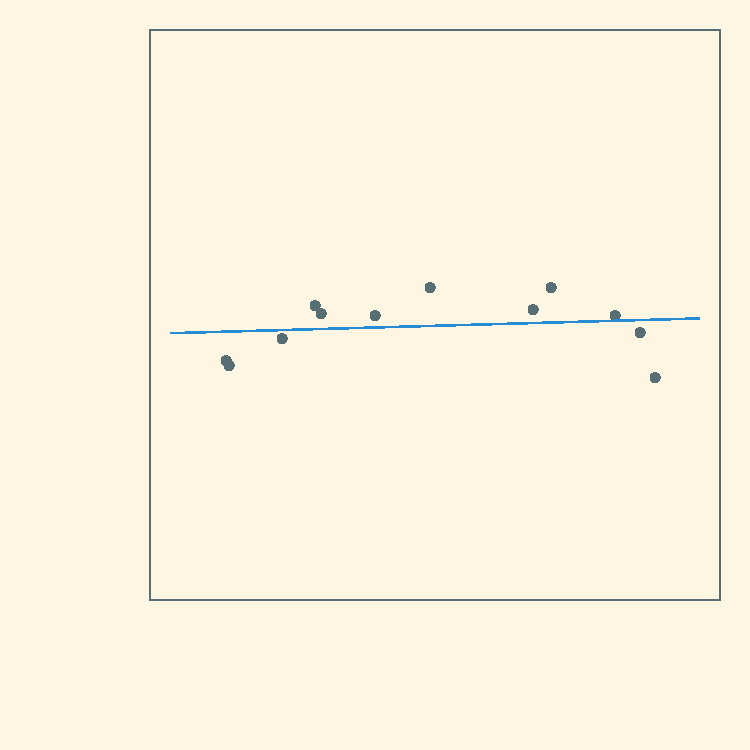
\includegraphics[width=\textwidth]{fig/train_linear}
    %     \caption{Linear Fit}
    % \end{subfigure}%
    % ~
    % \begin{subfigure}[t]{0.33\textwidth}
    %     \centering
    %     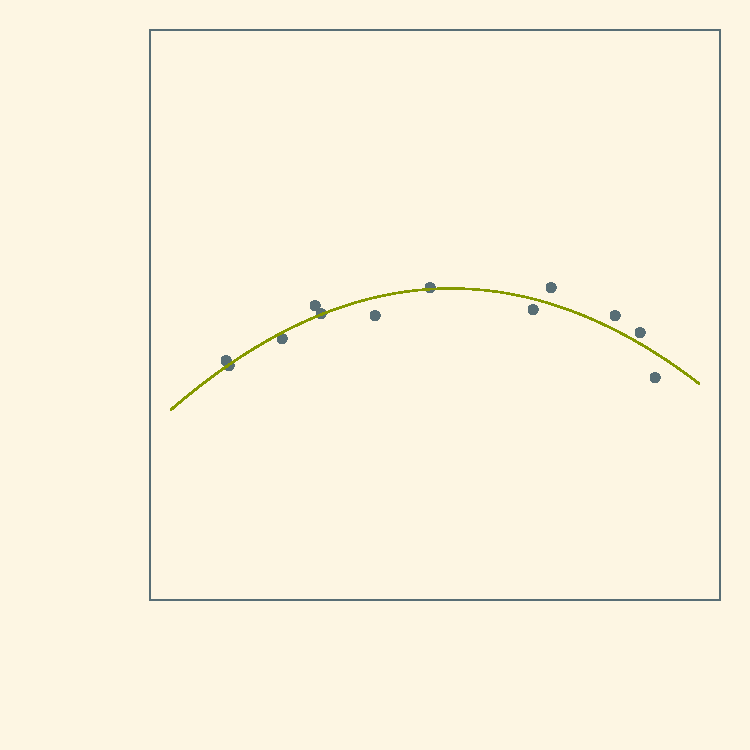
\includegraphics[width=\textwidth]{fig/train_quadratic}
    %     \caption{Quadratic Fit}
    % \end{subfigure}%
    % ~
    % \begin{subfigure}[t]{0.33\textwidth}
    %     \centering
    %     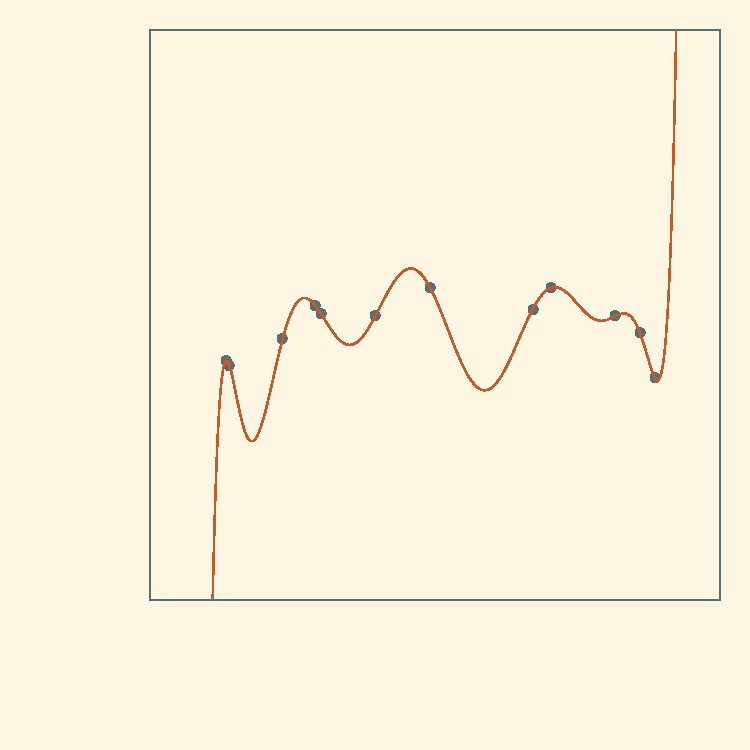
\includegraphics[width=\textwidth]{fig/train_overfit}
    %     \caption{Tenth-Order Fit}
    % \end{subfigure}
    \begin{subfigure}[t]{0.33\textwidth}
        \centering
        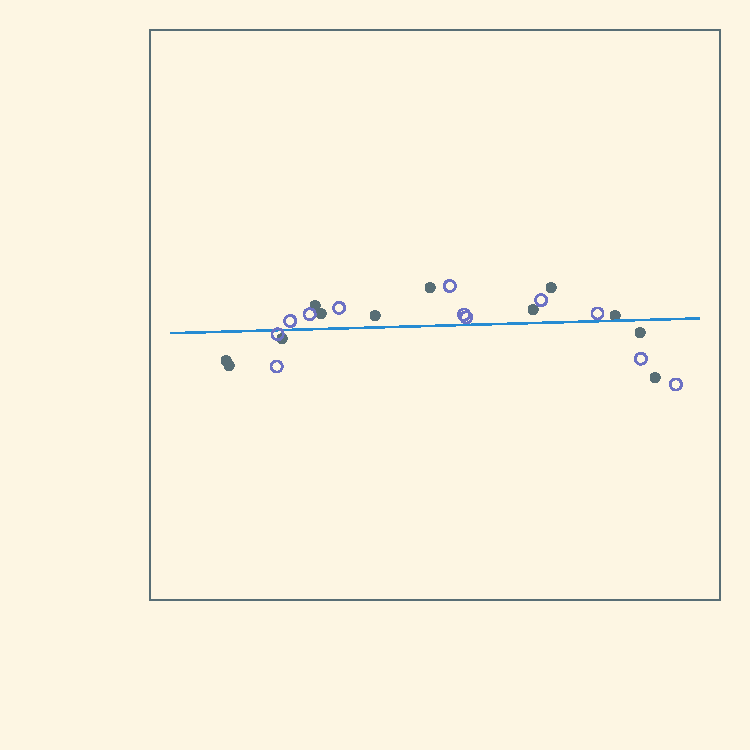
\includegraphics[width=\textwidth]{fig/test_linear}
        \caption{Linear Fit \label{fig:poly-linear}}
    \end{subfigure}%
    ~
    \begin{subfigure}[t]{0.33\textwidth}
        \centering
        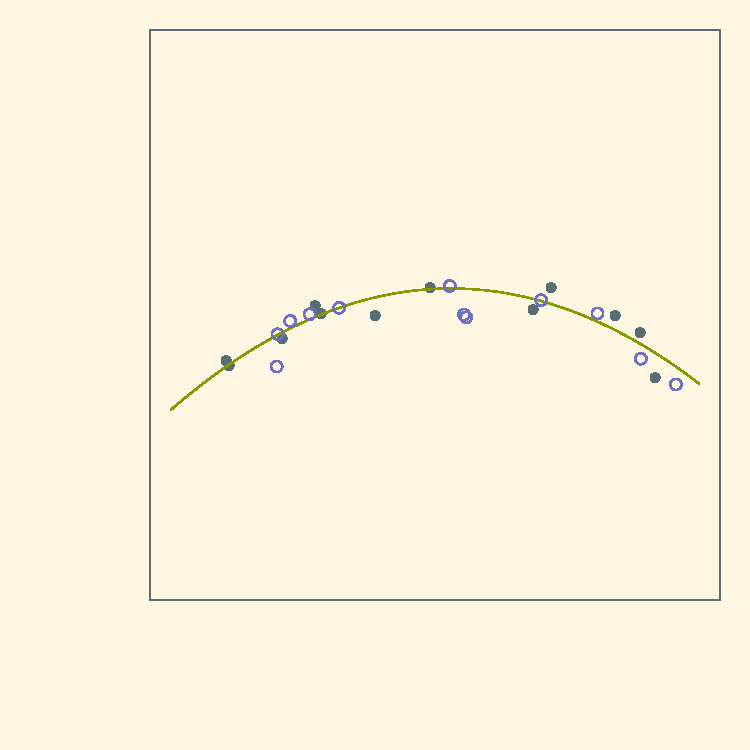
\includegraphics[width=\textwidth]{fig/test_quadratic}
        \caption{Quadratic Fit \label{fig:poly-quad}}
    \end{subfigure}%
    ~
    \begin{subfigure}[t]{0.33\textwidth}
        \centering
        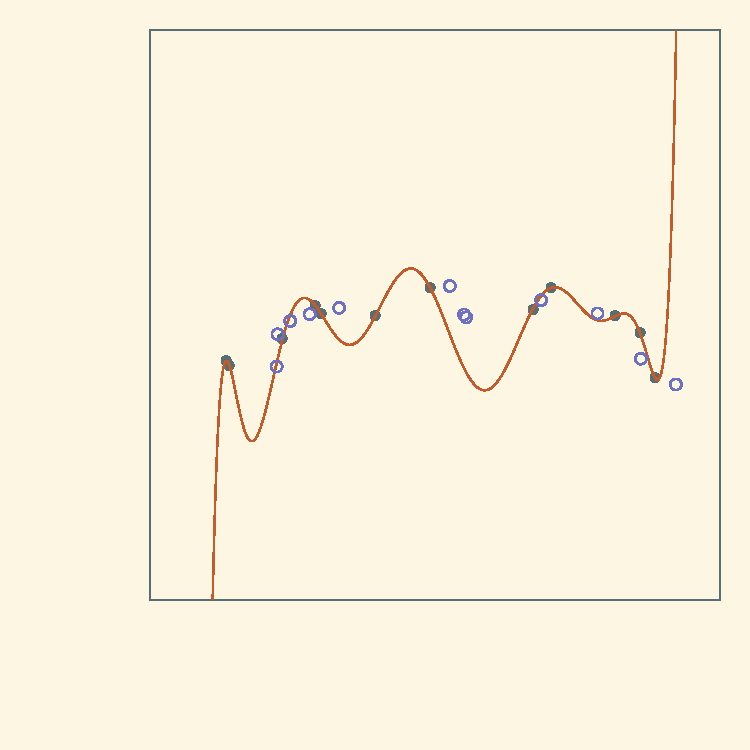
\includegraphics[width=\textwidth]{fig/test_overfit}
        \caption{Tenth-Order Fit \label{fig:poly10}}
    \end{subfigure}
    \begin{subfigure}[t]{0.5\textwidth}
        \centering
        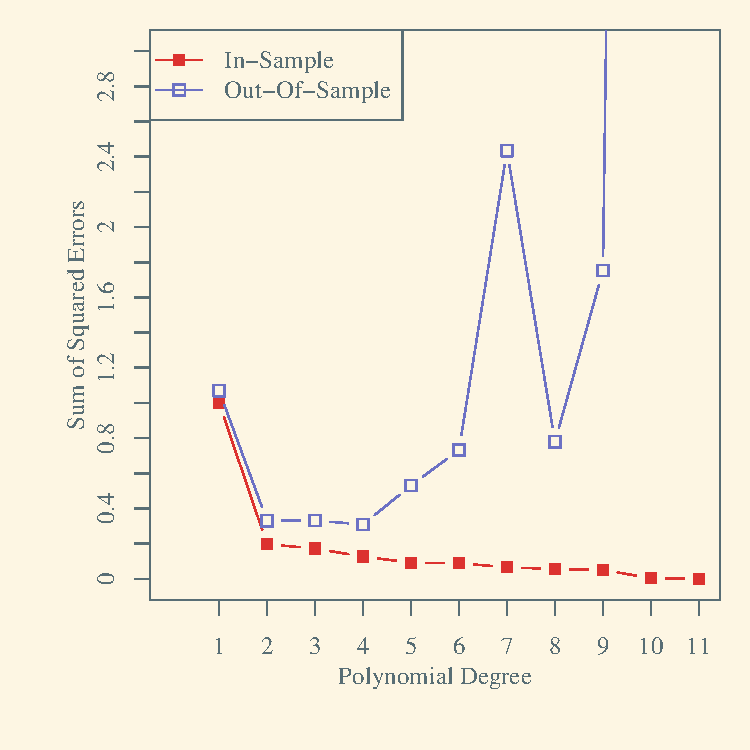
\includegraphics[width=\textwidth]{fig/poly_errors}
        \caption{Errors on Training and Test Set \label{fig:poly-errors}}
    \end{subfigure}
    \caption{\label{fig:polynomials} Polynomials of varying degrees fit using ordinary least
      squares (equivalently, maximum likelihood estimation) 
      to a set of eleven points generated from a fifth order
      polynomial with independent Normal
      residuals. \ref{fig:poly-linear}--\ref{fig:poly10}: fits of
      polynomial order 1, 2 and 10.  Filled circles are training data,
    unfilled circles are data not used during fitting.
    \ref{fig:poly-errors} squared prediction error in and out of the
    training sample for polynomial orders 1 through 10.}
\end{figure*}

\subsection{Balancing Fit and Complexity: Bayesian Occam's Razor}
\label{sec:balanc-fit-compl}

How do we go about deciding how complex a model to use in a given
setting?  One common approach is to use a penalized fit statistic, in
which the specific model $f$ is chosen not to maximize raw fit to the
data (e.g., by maximizing the likelihood), in which case more complex
models that contain simpler models as special cases will always be
chosen, but instead to maximize a {\em penalized} objective function
that balances in-sample fit with some measure of complexity.  This
complexity penalty can be viewed as a means to hold down the variance
of the model class; i.e., to combat overfitting.

Some examples of penalized fit measures that serve to select a subset
of predictor variables to receive nonzero coefficients in linear
regression are the lasso ($L_1$-penalized regression), Mallow's $C_p$,
and various ``information criteria'' such as AIC and BIC (TODO: ADD
CITATIONS).

Bayesian inference provides an alternative approach.  Whereas the
likelihood function serves as a measure of how surprising the data is given a fully
specified model, Bayesian inference provides a method for quantifying
how surprising the data and the specific model are together, where the
data is assumed to be selected stochastically from a set of possible
datasets allowed by the model (as in maximum likelihood estimation),
and additionally, the {\em model} is treated as though it were
selected stochastically from a set of possible models.  At each of
these choice points, if there are lots of options, any one of them
becomes more surprising.  

Consider the problem of choosing between two model
classes, $\mathcal{M}_1$ and $\mathcal{M}_2$, where $\mathcal{M}_1$
has no free parameters, and $\mathcal{M}_2$ has a free parameter
$\theta$, and reproduces $\mathcal{M}_1$ for a particular setting of
$\theta = \theta_*$.  The likelihood function by itself gives us no way by
itself to adjudicate between the two equivalent models,
$\mathcal{M}_1$ on the one hand, and $\mathcal{M}_2$ with $\theta =
\theta_*$ on the other since, $p(Y \given \mathcal{M}_1) = p(Y
\given \mathcal{M}_2, \theta_*)$.  Bayes' rule yields
\begin{align}
  p(\mathcal{M}_1 \given Y)&= \frac{p(\mathcal{M}_1) p(Y \given
    \mathcal{M}_1)}{p(Y)} \\
  p(\mathcal{M}_2 \given Y)&= \frac{p(\mathcal{M}_2) p(Y \given \mathcal{M}_2)}{p(Y)}
\end{align}
where in the case of $\mathcal{M}_2$, we need to expand the likelihood
to
\begin{equation}
  \label{eq:2}
  p(Y \given \mathcal{M}_2) = \int_{\Theta} p(Y \given \theta,
  \mathcal{M}_2) p(\theta \given \mathcal{M}_2) d\theta
\end{equation}
which is a weighted average of specific likelihoods of the form $p(Y
\given \theta, \mathcal{M}_2)$ with weights given by some distribution
over the parameter space.  Thus, if $\mathcal{M}_1$ assigns a large
likelihood to the observed data, even if $\mathcal{M}_2$ can achieve
the same likelihood at $\theta_*$, the ``good value'' $\theta_*$ will
be diluted in the {\bf marginal likelihood}, $p(Y
\given \mathcal{M}_2)$.

Hence, unlike maximum likelihood, 
Bayes theorem will tend to ``reward'' more restrictive {\em model
  classes} even in the case that the more flexible model contains the
simpler one as a special case, providing a built in Occam's Razor.
Of course, if there is some $\theta$ other than $\theta_*$ for which
the likelihood is greater, then $\mathcal{M}_2$ may win out depending
on whether the benefit to the likelihood outweighs the ``penalty''
induced by the $p(\theta \given \mathcal{M}_2)$ term, which is what we
want to happen, since the simplest model is only to be preferred if it
does about as good a job accounting for the data as the more complex model.

I now turn to the example of clustering a set of observations into
some number of groups, or, similarly, of fitting a mixture
distribution to a dataset.  I will introduce this problem in some
detail, since it is closely related to the main topic of this
dissertation, namely Hidden Markov Models, which I will introduce in
the following section, and treat in more detail in
Chapter \ref{chapter:HMM-NPBayes}.  I introduce the clustering
application here since it helps to motivate the bigger picture idea of
a nonparametric model.

\section{Clustering via a Mixture of Gaussians Model}
\label{sec:clustering}

Suppose we have a model of the form
\begin{equation}
  \label{eq:gmm}
  f(y \given \pi, \theta) = \sum_{k=1}^\infty \pi_k f(y \given \theta_k)
\end{equation}
where $\theta = (\theta_1, \theta_2, \dots)$ are some parameters
governing the mixture components, and $\pi = (\pi_1, \pi_2, \dots)$ is
the vector of mixing weights that sum to 1.

We could take a Bayesian approach and put priors on the vector of
mixture weights $\pi$ and on each
$\theta_k$.

Concretely, suppose that $f$ is Normal, so that $\theta_k = (\mu_k,
\sigma^2_k)$, and first suppose that we use a prior on $\pi_k$ that
fixes the number of nonzero weights to a finite value, $K$.  
Then the model is of the form
\begin{equation}
  f(y \given \pi, \theta) = \sum_{k=1}^K \pi_k \Norm{\mu_k}{\sigma^2_k}
\end{equation}

The $\pi_i$ define a categorical distribution over $K$ categories.
The categorical family has the conjugate prior
\begin{equation}
  f(\pi \given \xi) \propto \prod_{k=1}^K \pi_k^{\xi_k - 1}
\end{equation}
which is a {\bf Dirichlet distribution}.

We can also place conjugate priors on the $\mu_k$ and $\sigma_k$, such
as Normal and Inverse-Gamma, in the case of Normal components.

(Note that when $y$ is vector valued, $\mu$ becomes a mean vector and
$\sigma^2$ becomes a covariance matrix.  It is also possible to define
conjguate priors for these.)

Putting everything together and assuming Normal components, we have the joint prior:
\begin{equation}
  f(\pi, \mu, \sigma^{-2}) \propto \prod_{k=1}^K \pi_k^{\xi_k - 1}
  e^{-\frac{1}{2\sigma_k^2} (\mu_k
  - \mu_0)^2} \sigma_k^{-2a_0 - 2} e^{-\sigma_k^{-2} b_0}
\end{equation}
and the joint likelihood
\begin{equation}
  f(y \given \pi, \mu, \sigma^2) = \prod_{i=1}^n \sum_{k=1}^K \pi_k
  \sigma_k^{\frac{1}{2}} e^{-\frac{1}{2\sigma_k^2}(x_i - \mu_k)^2}
\end{equation}

That sum is trouble for inference.  
What we can do is to represent the likelihood in two stages: instead
of saying that each $y_i$ is drawn from a weighted mixture of the $K$
components, we can instead say that each $y_i$ comes from precisely
one component; we just do not know which one.  However, we can say
that $y_i$ comes from component $k$ with probability $k$.  We can
imagine generating data as follows:

For each $i = 1, \dots, n$
\begin{enumerate}
\item Draw $z_i \sim \mathrm{Categorical}(\pi_1, \dots, \pi_K)$
\item Draw $y_i \sim f(y \given \mu_{z_i}, \sigma^2_{z_i})$
\end{enumerate}

The joint likelihood for the $z_i$ and $y_i$ becomes
\begin{align}
  f(z_i, y_i \given \pi, \mu, \sigma^2) = f(z_i \given \pi) f(y_i
  \given z_i, \mu, \theta) &\propto \prod_{i=1}^n \pi_{z_i}
  (\sigma^2_{z_i})^{-1/2} e^{-\frac{1}{2\sigma^2} (y_i - \mu_{z_i})^2}\\
  &= \prod_{k=1}^K \pi_k^{n_k} (\sigma_k^2)^{-\frac{n_k}{2}}
  e^{-\frac{1}{2\sigma^2_k} \sum_{i: z_i = k} (y_i - \mu_k)^2}
\end{align}
which yields a posterior distribution with simple conditional
distributions that can be sampled from very straightforwardly using a
Gibbs sampler, in which the set of posterior variables is divided into
blocks, each of which is iteratively sampled from its conditional
posterior given the previous state of the others, which defines a
Markov Chain whose stationary distribution is the full posterior 
\citep{geman1984stochastic}.

\section{Clustering Sequential Data: The Hidden Markov Model}

In many applications, data are not i.i.d., but have some known
dependence structure.  Sequential data is one such case.  Suppose a
dataset consists of an ordered sequence of observations, ${y_t}, t =
1, \dots, T$.  Since unlike in the i.i.d. case we assume the order is
meaningful (most typically, the index $t$ might represent the time at which the data
point was collected), it is reasonable to expect that observing the
value at time $t$ would alter the predictive distribution at time
$t+1$, even if we knew the marginal distribution.  For example, $y_t$
might be a word or a sentence of text in a document, a snippet of a
sound recording, physiological measurements collected over time.  In
all of these cases, we expect nearby observations either to be
similar, or to be made more predictable given the last few observations.

One option would be to encode the dependencies among the data points
through a conditional model of the data at time $t$ given various
combinations of data at time $t-1$, $t-2$, \dots, $t-s$; that is, to
model the data using an order $s$ Markov chain. However, modeling the
distribution conditioned directly on observations risks an overly
complex conditioning structure, since in most settings there is likely
to be some idiosyncratic noise present in each observation that does
not depend on time in the same way as the underlying signal.  That is,
quite often the distribution at $t$ is likely to be a mixture of a temporally dependent
component and a temporally independent component.

The {\bf Hidden Markov Model}, first developed by
\citet{baum1966statistical} (see also \citet{rabiner1986introduction}
for a classic tutorial) separates temporal dynamics of an evolving
underlying (``hidden'') state from an temporally independent ``noise''
component by augmenting the observed time sequence $\{y_t\}, t = 1,
\dots, T$ with a latent data sequence, $\{z_t\}, t = 1,
\dots T$, such that at the distribution of the observations, $y_t$ are
independent conditioned on the latent sequence, $z_t$, but the $z_t$
evolve according to a Markov chain.  More formally, the model is
\begin{align}
  z_1 &\sim \Cat{\pi_{01}, \dots, \pi_{0J}} \\
  z_t \given z_{t-1} &\sim \Cat{\pi_{z_{t-1}1}, \dots,
    \pi_{z_{t-1}J}}, \quad t = 2, \dots, T
  \\
  y_t \given z_t &\sim F(\theta_{z_t}), \quad t = 1, \dots, T
\end{align}

where the vector $\pi_0 = (\pi_{01}, \dots, \pi_{0K})$ is the initial
distribution of the underlying Markov chain, the matrix $(\pi_{jj'}),
j,j' = 1, \dots, J$ is the transition matrix of the Markov chain, $F$
is a family of {\bf emission distributions}, which is parameterized
for each state in the Markov chain by the $\theta_j, j = 1, \dots, J$.

This model is nearly identical to the mixture model discussed in
Sec. \ref{sec:clustering}, the only difference being the dependence of
the label, $z_t$ on the previous label, $z_{t-1}$.  We can indeed
construct an easy to work with Bayesian HMM by placing an appropriate 
conjugate prior on the $\theta_t$ emission parameters (e.g.,
Normal-Inverse Wishart in the case where $F$ is the family of Normal
distributions), and Dirichlet conjugate priors on $\pi_0$ and 
on each row of $\pi$, and carry out posterior inference using Gibbs
sampling: alternating between sampling the state sequence $\{z_t\}$
and the model parameters, $\pi, \pi_0$ and the $\theta_j$.  There is
some additional difficulty introduced by the fact that the $z_t$
indicators are no longer conditionally independent, and so we must
either sample them jointly, or break up the Gibbs sampler into
many additional blocks so as to sample each $z_t$ conditioned on all
the others.  I will defer details of inference in this model until
Chapter \ref{chapter:HMM-NPBayes}.


\section{Model Selection in HMMs and the Mixture of Gaussians Model}
\label{sec:model-select-mixt}

It is relatively rare that we would be in a situation where we wanted
to fit a mixture of Gaussians to a dataset and knew exactly how many
components there were in the mixture.  It is perhaps somewhat more
likely that we know in advance how many
states the hidden Markov chain in an HMM can visit, but there are
certainly settings where we cannot or would not wish to do this. 
What can we do if we cannot specify $K$ ahead of time?

One approach is to apply the logic outlined in
Sec. \ref{sec:balanc-fit-compl} and simply put a prior distribution on
$K$, and then calculate (or sample from) the posterior distribution
over $K$.  Then, although we can always achieve at least as large a
likelihood with a larger $K$ as with a smaller $K$ (either by setting
some mixture weights to zero, or by effectively combining multiple
components into one by creating mixture components with
identical means and variances), since models with larger $K$ have more flexibility, their
marginal likelihood will tend to be diluted by all of the ways they can fit
the data badly.

However, this requires doing inference separately for as many values
of $K$ as we want to consider, and for the larger values of $K$, this
inference can be computationally expensive.  It turns out that we can
achieve substantially the same thing more simply by employing a single
{\bf nonparametric} model with an {\em infinite} number of
components.  

In the next chapter, I turn to the distinction between parametric and
nonparametric models, develop some of the theory of {\bf Dirichlet Process Mixture
  Models}, which form the basis for the infinite-state Hidden Markov
Model, which I define after that, along with additional detail on
Gibbs sampling in these two models.

% In Chapter \ref{chapter:HaMMLeT}, I introduce a new model, the Hidden
% Markov Model with Local Transitions (HaMMLeT), which generalizes the
% infinite state Hidden Markov Model to allow more specific prior
% information on the state space to be incorporated.  Then, in Chapters
% \ref{chapter:cocktail-party} through Chapter \ref{chapter:music}, I
% define variations on the basic HaMMLeT model in order to test the
% model on several kinds of data.  Finally in Chapter
% \ref{chapter:discussion} I give some concluding thoughts and outline
% plans for future work.
